% remember to set these at the start of each chapter
\chapter{Background} 
\label{background} 

\section{Neural Networks}

The term Neural Network (NN) refers to a computational model that is artificially built in computers. The artificial Neural Network is inspired by the way biological neural networks in the human brain process information. Artificial Neural Networks have generated a lot of excitement in Machine Learning research and industry, thanks to many breakthrough results in speech recognition, computer vision and text processing. In this section, we will discuss the fundamentals of a Neural Network.

\subsection{A Single Neuron}
Neuron, or node, is a basic computation unit in NN. It simply takes some inputs $(x_1,...,x_n)$ and computes an output Y. Each input has an associated weight $(w_1,...,w_n)$, which is assigned on the basis of its relative importance to other inputs. The node applies a function $f$ to the weighted sum of its inputs (and a bias term $b$). The output of a node is $f(w_1 \cdot x_1 +...+ w_n \cdot x_n + b)$, shown in Fig.\,\ref{node}.
\begin{figure}
	\centering
	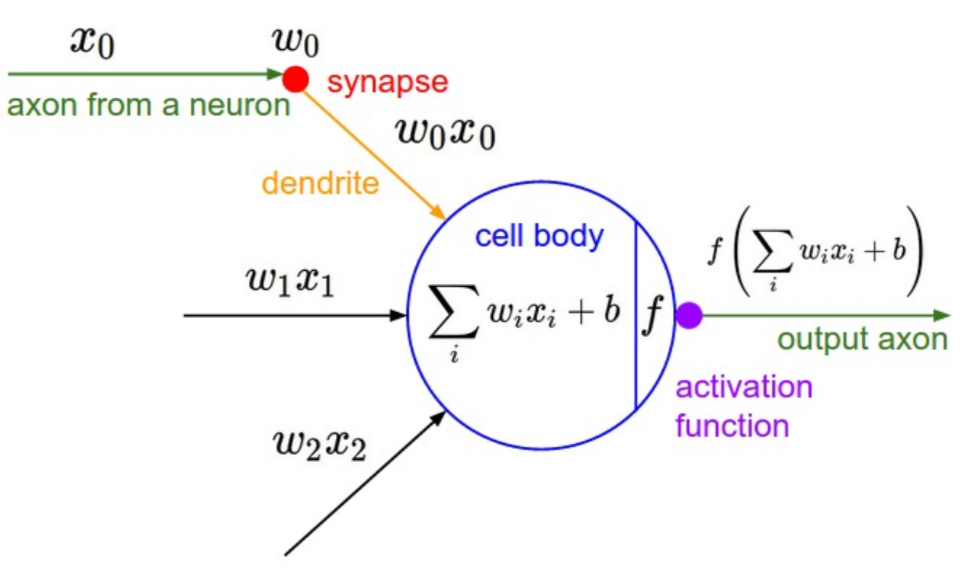
\includegraphics[scale=0.5]{Figs/node.png}
    \caption{A Node}
    \label{node}
\end{figure}

The function $f$ is non-linear and is called the Activation Function. The purpose of the activation function is to introduce non-linearity into the output of a node. The following activation function (Fig.\,\ref{activation}) is often used:
\begin{figure}
	\centering
	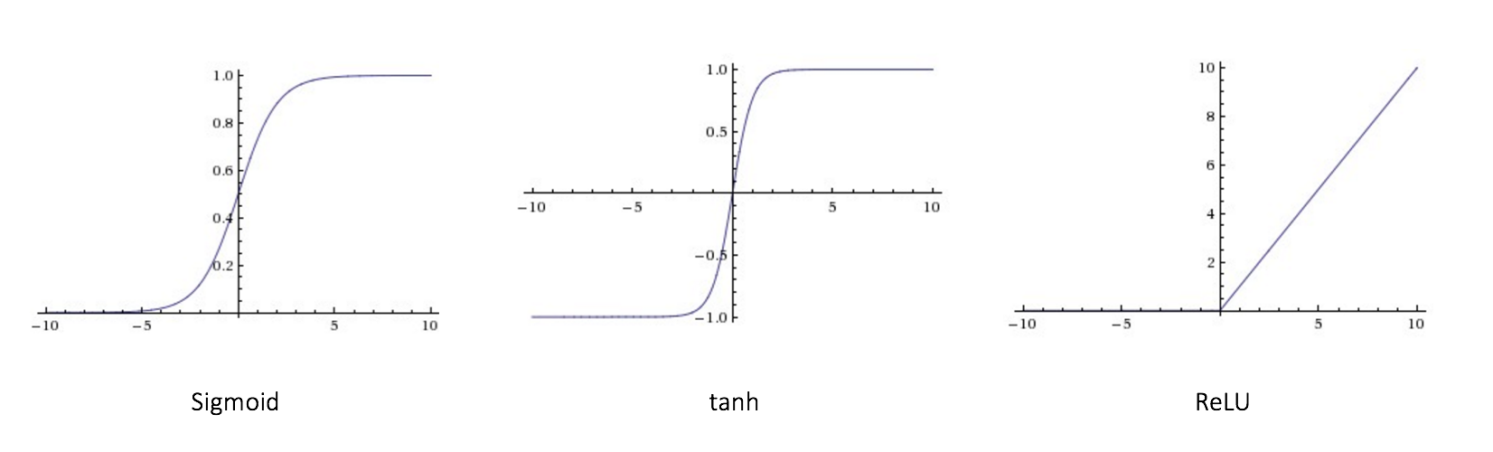
\includegraphics[scale=0.5]{Figs/activation.png}
    \caption{Activation Functions}
    \label{activation}
\end{figure}

\begin{itemize}
  \item Sigmoid: takes a real-valued input and squashes it to range between 0 and 1
        $$ \sigma(x) =  \frac{\mathrm{1} }{\mathrm{1} + e^{-x} }  $$ 
  \item tanh: takes a real-valued input and squashes it to the range [-1, 1]
        $$ tanh(x) = 2\cdot\sigma(2x)-1 $$
        
  \item ReLU(Rectified Linear Unit): takes a real-valued input and thresholds it at zero
        $$f(x) = \max(0,x)$$
\end{itemize}

\subsection{Feedforward Neural Network}

The simplest Neural Network is a feedforward fully connected network. It is formed by one or multiple layers of nodes. Nodes in adjacent layers have connections between them. A connection represents a set of weights.


\noindent An example of a feedforward neural network is shown in Fig.\,\ref{feedforward}.
\begin{figure}[h]
	\centering
	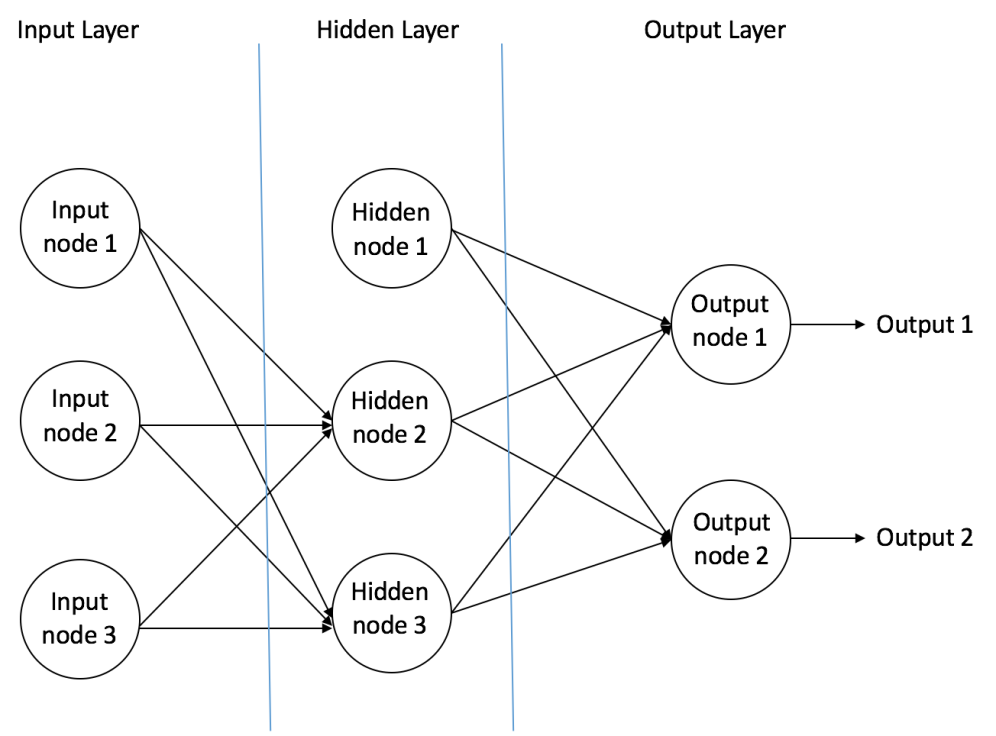
\includegraphics[scale=0.5]{Figs/feedforward.png}
    \caption{Feedforward Neural Network}
    \label{feedforward}
\end{figure}

A feedforward neural network can consist of three types of nodes:

\begin{enumerate}
\item Input Nodes – The Input nodes take in a input $X$ in the form of vector $(x_1,...,x_n)$. These nodes are together referred to as the “Input Layer”. No computation is performed in any of the Input nodes – they just pass on the information to the hidden nodes.

\item Hidden Nodes – The Hidden nodes are in between Input Layer and Output Layer. They have no direct connection with the network input and the network output, thus they are called "Hidden" and form "Hidden Layer". After training, Hidden Node will learn some relationship (non-linearality) between its input and output. A feedforward network can have zero, one, or multiple Hidden Layers.

\item Output Nodes – The Output nodes are collectively referred to as the “Output Layer” and are responsible for computations and producing output from the "Hidden Layer". Output Layer works in similar way as a Hidden Layer, but the output of this layer is considered the final output of the network.

\end{enumerate}

In a feedforward network, the information moves in only one direction – forward – from the input nodes, through the hidden nodes and to the output nodes. There are no cycles or loops in the network.


\subsection{Multi Layer Perceptron}
A Multi Layer Perceptron (MLP) contains one or more hidden layers (apart from one input and one output layer).  While a single layer perceptron can only learn linear functions, a multilayer perceptron can also learn non-linear functions.

Fig.\,\ref{mlp} shows a multilayer perceptron with a single hidden layer. Note that all connections have weights associated with them, but only three weights $(w_1,...,w_n)$ are shown in the figure.

\begin{figure}[h]
	\centering
	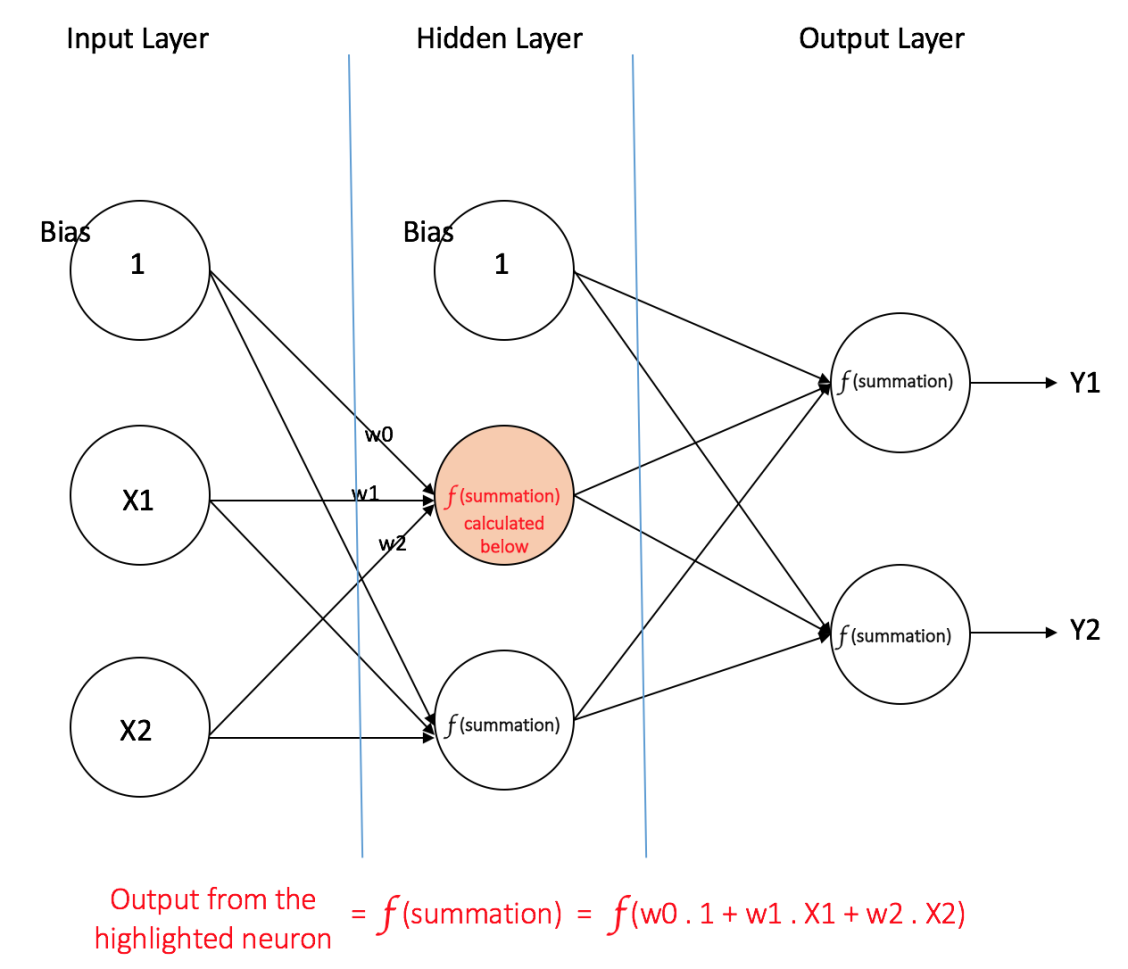
\includegraphics[scale=0.5]{Figs/multilayer.png}
    \caption{Multi Layer Perceptron}
    \label{mlp}
\end{figure}

\textbf{Input Layer}: The Input layer has three nodes. The Bias node has a value of 1. The other two nodes take in the input $X = (x_1,x_2)$. These values form the Input Layer and are passed to the Hidden Layer.

\textbf{Hidden Layer}: The Hidden layer also has three nodes with the Bias node having an output of 1. The output of the other two nodes in the Hidden layer depends on the Input layer $(b, x_1, x_2)$ as well as the weights $(w_0,w_1,...,w_n)$ associated with the connections (edges). Fig.\,\ref{mlp} shows the output calculation for one of the hidden nodes (highlighted). $Y_{Node} = f(\sum{w_0+w_1x_1+w_2x_2})$, where $f$ is an activation function.

\textbf{Output Layer}: The Output layer has two nodes which take inputs from the Hidden layer and perform similar computations as shown for the highlighted hidden node. The values calculated $(y_1,y_2)$ as a result of these computations act as output $\hat{y}$ of the Multi Layer Perceptron.

Given a set of features $X = (x_1,...,x_n)$ and a target $y = (y_1,..,y_n)$, a Multi Layer Perceptron can learn the relationship between the features and the target, for either classification or regression.


\subsection{Back-Propagation}
Back-Propagation refers to the backward propagation of errors. A Neural Network learns through Back-Propagation by calculating the error from the output $\hat{y}$ to the true value $y$, then improving the weights in all nodes. The learning is "supervised", meaning the true value $y$ must be known respect to each input $X$.



\section{Convolutional Neural Networks}
\subsection{Convolution Layer — The Kernel}
\subsection{Pooling Layer}
\subsection{Classification — Fully Connected Layer (FC Layer)}
\section{K-Fold Cross Validation}
\section{Image data augmentation}



